\begin{frame}
  \frametitle{Feature importance}
  \begin{itemize}
    \item Many ways to define \emph{importance}
    \item Permutation Feature Importance (PFI)
    \item What is the accuracy drop if we exclude/permute/randomize a feature?
  \end{itemize}
\end{frame}


\begin{frame}
  \frametitle{Permuation Feature Importance (PFI)}
  \begin{figure}
    \centering
    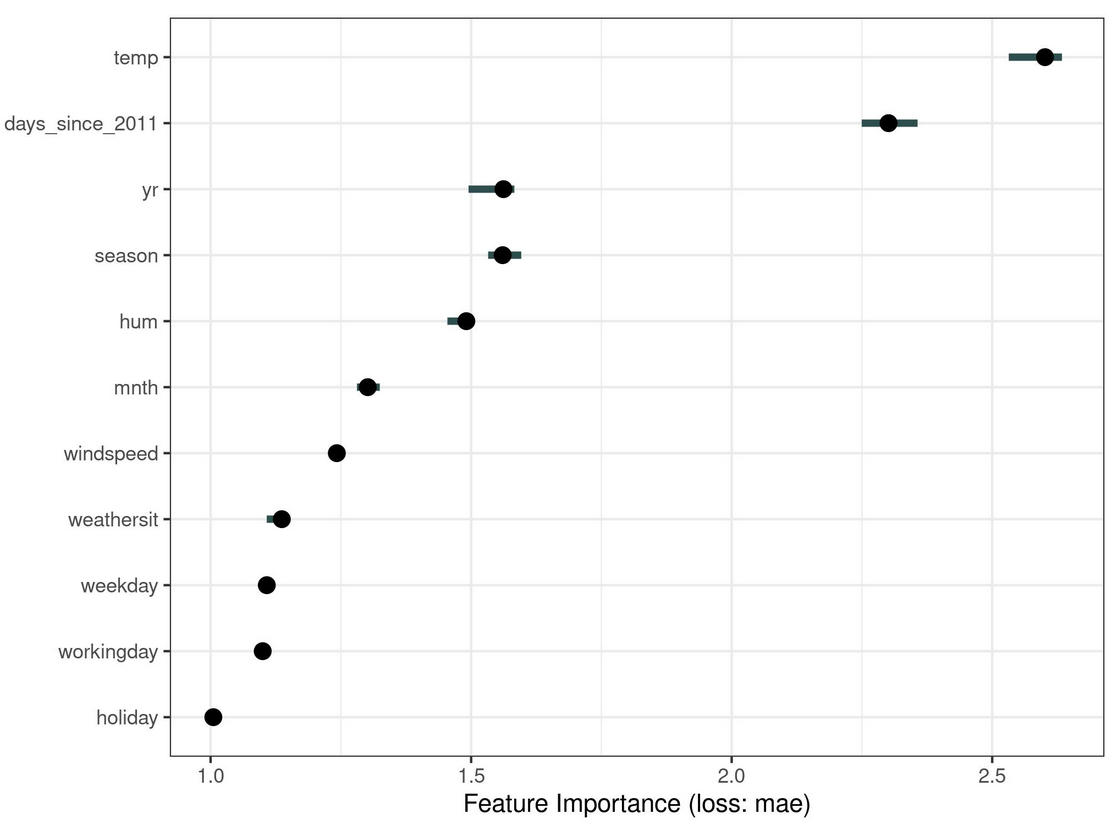
\includegraphics[width=0.8\linewidth]{pfi}
    \caption{Image taken from \href{https://christophm.github.io/interpretable-ml-book/feature-importance.html}{Interpretable Machine Learning}}
  \end{figure}
\end{frame}


\begin{frame}
  \frametitle{Challenges/ideas for feature importance}
  \begin{itemize}
    \item Other ideas:
    \begin{itemize}
      \item Connection with feature effect
      \item $\mathtt{FI}_s = \int_{x_s} f_s(x_s)$, i.e.~energy of the signal
    \end{itemize}
    \item Challenges:
    \begin{itemize}
      \item Just permute the feature and measure the accuracy or retrain on the permuted dataset?
      \item If just permute, two highly correlated features may divide their importance (seem less important)
      \item If just permute, we suffer from unrealistic instances
      \item If retrain, two highly correlated features may cover each other (seem unimportant)
    \end{itemize}
  \end{itemize}
\end{frame}



